\documentclass[sigconf]{acmart}

\usepackage{booktabs} % For formal tables
\usepackage[normalem]{ulem}
\usepackage{soul,color}
\usepackage{listings}
\usepackage{tikz}
\usetikzlibrary{arrows,decorations.pathmorphing,backgrounds,fit,positioning,shapes.symbols,chains,shapes.geometric,shapes.arrows,calc}
% Copyright
\setcopyright{none}

\usepackage{ifthen}
\usepackage[normalem]{ulem} % for \sout
\usepackage{xcolor}
\usepackage{amssymb}

\newcommand{\ra}{$\rightarrow$}
\newboolean{showedits}
\setboolean{showedits}{true} % toggle to show or hide edits
\ifthenelse{\boolean{showedits}}
{
	\newcommand{\ugh}[1]{\textcolor{red}{\uwave{#1}}} % please rephrase
	\newcommand{\ins}[1]{\textcolor{blue}{\uline{#1}}} % please insert
	\newcommand{\del}[1]{\textcolor{red}{\sout{#1}}} % please delete
	\newcommand{\chg}[2]{\textcolor{red}{\sout{#1}}{\ra}\textcolor{blue}{\uline{#2}}} % please change
}{
	\newcommand{\ugh}[1]{#1} % please rephrase
	\newcommand{\ins}[1]{#1} % please insert
	\newcommand{\del}[1]{} % please delete
	\newcommand{\chg}[2]{#2}
}

\newboolean{showcomments}
\setboolean{showcomments}{true}
%\setboolean{showcomments}{false}
\newcommand{\id}[1]{$-$Id: scgPaper.tex 32478 2010-04-29 09:11:32Z oscar $-$}
\newcommand{\yellowbox}[1]{\fcolorbox{gray}{yellow}{\bfseries\sffamily\scriptsize#1}}
\newcommand{\triangles}[1]{{\sf\small$\blacktriangleright$\textit{#1}$\blacktriangleleft$}}
\ifthenelse{\boolean{showcomments}}
%{\newcommand{\nb}[2]{{\yellowbox{#1}\triangles{#2}}}
{\newcommand{\nbc}[3]{
 {\colorbox{#3}{\bfseries\sffamily\scriptsize\textcolor{white}{#1}}}
 {\textcolor{#3}{\sf\small$\blacktriangleright$\textit{#2}$\blacktriangleleft$}}}
 \newcommand{\version}{\emph{\scriptsize\id}}}
{\newcommand{\nbc}[3]{}
 \renewcommand{\ugh}[1]{#1} % please rephrase
 \renewcommand{\ins}[1]{#1} % please insert
 \renewcommand{\del}[1]{} % please delete
 \renewcommand{\chg}[2]{#2} % please change
 \newcommand{\version}{}}
\newcommand{\nb}[2]{\nbc{#1}{#2}{orange}}

\definecolor{accolor}{rgb}{0.4,0.6,0.2}
\newcommand\ac[1]{\nbc{AC}{#1}{accolor}}
\usepackage{wasysym}
\newcommand\yesml[1]{\nbc{ML {\textcolor{yellow}\sun}}{#1}{mircolor}}

\definecolor{sgcolor}{rgb}{0.2,0.0,0.5}
\newcommand\sg[1]{\nbc{SG}{#1}{sgcolor}}

\definecolor{frcolor}{rgb}{0.2,0.4,0.2}
\newcommand\fr[1]{\nbc{FR}{#1}{frcolor}}

\definecolor{bbcolor}{rgb}{0.21,0.54,0.84}
\newcommand\bb[1]{\nbc{BB}{#1}{bbcolor}}

% Todo Command
\definecolor{todocolor}{rgb}{0.9,0.1,0.1}
\newcommand{\todo}[1]{\nbc{TODO}{#1}{todocolor}}



\begin{document}

\title{BlueBridge: Pushing Shared Memory Management into the Network}


\author{Fabian Ruffy}
\affiliation{%
  \institution{University of British Columbia}
}
\email{fruffy@cs.ubc.ca}

\author{Amanda Carbonari}
\affiliation{%
  \institution{University of British Columbia}
}
\email{acarb95@cs.ubc.ca}

%%%%%%%%%%%%%%%%%%%%%%%%%%%%%%%%%TO DO%%%%%%%%%%%%%%%%%%%%%%%%%%%%%%%%%
% 1. Fix citations --> shouldn't always be in line (see Related Works)
%%%%%%%%%%%%%%%%%%%%%%%%%%%%%%%%%%%%%%%%%%%%%%%%%%%%%%%%%%%%%%%%%%%%%%%


\begin{abstract}
% \fr{needs work}
% With the onsets of cheaper memory, datacenters can now house denser memory servers. This changes how applications can leverage in-memory processing, they now have a large bank of memory available to them. A distributed shared memory system can aid in the development of these applications by providing a single virtual address space for the application to operate on. But, distributed shared memory's main disadvantages are the complexity of concurrency, complexity of tracking data migration, and communication overhead. Current network trends, such as RDMA and Infiniband, reduce the overhead of communication, which leaves the complexity of management as the main blocking factor for distributed shared memory systems.  

Distributed shared memory (DSM) systems have been well explored, but never managed to reach widespread adoption due to the complexity involved in building them. Instead of attempting to use or build a complex DSM system, programmers opted to control the messaging semantics of their applications. An increasing trend of in-memory computation and change in datacenter programming models has led to a resurgence of DSM. Disaggregated racks require the application to reason about shared memory in order to leverage the large amount of memory in a dedicated server. DSM systems can improve the programmability of these applications, but all the management complexity inherent to DSM systems must still be addressed.

To mitigate this complexity, we propose BlueBridge, a network managed shared memory system which stores every memory address as an IPv6-compliant address. This allows the location information of memory to be encoded in the IPv6 header, which the switch can operate on, effectively moving the directory service to the switch. With the global knowledge of where memory resides and the traffic information, the controller can now manage access, migration, and concurrency of the memory.

We realize BlueBridge with an initial proof of concept implementation, which shows that IPv6 memory addressing is possible. When evaluating this implementation, we show that we can achieve a 2x reduction in latency per remote page access and, with RDMA, we can achieve latencies similar to local disk access. These numbers are not concrete representations of the speed up BlueBridge can achieve, rather they show the promise of what a fully optimized system can achieve. 
\end{abstract}

\keywords{Distributed Shared Memory, Software-Defined Networks, Remote Memory}


\maketitle

%%%%%%%%%%%%%%%%%%%%%%%%%%%%%%%%%%%%%%%%%%%%%
\section{Introduction}
\label{sec:intro}
%%%%%%%%%%%%%%%%%%%%%%%%%%%%%%%%%%%%%%%%%%%%%

Big data processing is complicated. Typically scientists, and
experienced programmers alike struggle with managing and configuring
clusters of machines to processes large amounts of data. Frameworks
like Hadoop and Pregal have significantly eased the difficulty of big
data processing, but they remain intimidating for the lay man. We
noticed a trend in non-systems scientists, and researchers, that they
wanted to \textit{"Just write python code that ran on a bunch of
computers"}. For the benefit of science we investigated how to make
this dream a reality.

Making all Python code run on clusters of machines is impractical, and
due to network overhead would lead to sluggish un-optimal code. Instead
we concentrated our efforts on a common, but difficult big data
processing task, graph processing. Many frameworks exist for
distributed graph
processing~\cite{Malewicz:2010:PSL:1807167.1807184,Ching:2015:OTE:2824032.2824077,Kyrola:2012:GLG:2387880.2387884,Low:2012:DGF:2212351.2212354,Xin:2013:GRD:2484425.2484427,Gonzalez:2012:PDG:2387880.2387883},
and many general frameworks exist which are used for graph
processing~\cite{Vavilapalli:2013:AHY:2523616.2523633,Zaharia:2012:RDD:2228298.2228301,Isard:2007:DDD:1272996.1273005,Murray:2013:NTD:2517349.2522738}.
These frameworks vary in their complexity, but none are
\textit{"accessible"} for programmers with no systems experience.

With the exception of~\cite{Kyrola:2012:GLG:2387880.2387884} the
aforementioned systems suffer a common pitfall to accessibility; they
expose the complexity of a distributed message passing system to the
user. Extensive work has been done to hide this complexity in the
abstraction of distributed shared memory (DSM)
~\cite{Keleher:1994:TDS:1267074.1267084,Power:2010:PBF:1924943.1924964,Morin:2004:KDP:1111682.1111729,Haddad:2001:MCL:374794.374800,Huang06vodca:view-oriented}.
The benefits of DSM have been ignored in recent years due its flaws,
mainly fate sharing and sub optimal performance. Dismissing DSM may
well have been a shortsighted mistake. Ultra dense memory, and the
approach of terabit bandwidth within a rack give modern racks the
appearance of single machines, and has lead towards disaggregated
architectures~\cite{facebook-rack,machine,intel-rsa,seamicro,Han:2013:NSR:2535771.2535778}.
Such futuristic systems lend themselves naturally to DSM which
motivates our proposal for a corresponding computation framework.

The largest disadvantage of DSM is performance. Programmers can write
terribly performant programs by failing to reason about the location
of memory, leading to memory thrashing. In computation where a high
degree of consistency between shared resources DSM is the wrong tool
for the job. In contrast when large amounts of computation can be
performed between memory synchronizations DSM provides a simple and
efficient programming model. Graph processing suffers from a lack of
locality. In computations such as PageRank a single iteration may
require edge updates which require the synchronization of every
machine in a cluster. This problem can be largely avoided in practice
by carefully pre-processing graphs into partitions where the minimum
number of graph edges cross machines. The cost of pre-processing a
graph can be large, in some cases the complexity of finding a good
partition is greater than solving the initial problem! Here we
demonstrate that the cost of graph partitioning is worth it for the
benefits that DSM provides.

In this paper we attack the problem of developing a simple and
efficient graph processing interface for DSM. Specifically we make the
following contributions.

\begin{itemize}
        \item A simple graph processing api
        \item A graph partitioning scheme optimal for DSM
        \item An evaluation of processing performance between partitioned DSM processing, and pregal style graph processing
\end{itemize}

The remainder of this paper is organized as follows. In
Section~\ref{sec:related} we over view related work. In
Section~\ref{sec:api} we describe our graph processing API.
Section~\ref{sec:partition} we describe our approach to graph
partitioning.In Section~\ref{sec:eval} we evaluate our framework
against a pregal style \textit{think like a vertex model}.
Section~\ref{sec:discussion} describes our experiences with our
system, and Section~\ref{sec:conclusion} concludes the paper.





% \section{Background}
\label{sec:background}

\begin{itemize}
    \item treadmarks~\cite{Keleher1994} \todo{Fabian} \\
    \item piccilo~\cite{piccolo} \todo{Fabian}  \\
    \item ramcloud~\cite{Ousterhout:2015:RSS:2818727.2806887} \todo{Stewart} \\
    \item distributed data processing (Hadoop~\cite{Dean2004}/pregal~\cite{Malewicz:2010:PSL:1807167.1807184}/spark~\cite{180560} \\ dryad~\cite{Isard:2007:DDD:1272996.1273005}/naiad~\cite{Murray:2013:NTD:2517349.2522738}) \todo{Stewart} \\
\end{itemize}

%%%%%%%%%%%%%%%%%%%%%%%%%%%%%%%%%%%%%%%%%%%%%%%%%%%%%%
\section{Related Work}%Do we want this to be at the beginning or end of the paper? Right now this reads more like motivation
\label{sec:related}
% \ugh{ASSIGNED TO: Amanda and Fabian}\\
%%%%%%%%%%%%%%%%%%%%%%%%%%%%%%%%%%%%%%%%%%%%%%%%%%%%%%
We categorize related work to BlueBridge in three categories: distributed shared memory systems, remote paging systems, and using Software Defined Networking for storage or memory.

\textbf{Distributed Shared Memory.} 
% \ac{Should include modern solutions $\rightarrow$ FARM}
% What solutions have been done and proposed in this space? Why is ours supposed to work better than theirs? 
Distributed shared memory has been explored extensively in previous decades~\cite{treadmarks, gms, Protic1996, Nitzberg1991, grappa, farm}. Our solution is similar to traditional distributed shared memory implementations but differs fundamentally in the management strategy. Therefore, we restrict our discussion of related works to the management components of distributed shared memory systems.

Two of the most recent systems are FaRM from Microsoft\cite{farm} and Grappa from University of Washington~\cite{grappa}. Both are similar to the traditional approaches described in~\cite{Protic1996, Nitzberg1991} but differ in the hardware used and design decisions. Both Grappa and FaRM take a more decentralized approach to their directory services. Each node is required to contact the ``owner'' of the memory in order to get routing information or to send requests~\cite{grappa, farm}. This solution tends to avoid the performance overheads from a centralized solution, but can perform poorly when memory migrates. Our solution differs as the memory address is the IPv6 location of the memory. The switch will map that IPv6 address to the correct machine which owns that piece of memory. In the case of memory migration, the controller will update the switch with new rules, thus re-routing the same IPv6 address to the new owner.

% Grappa has a similar approach as FaRM, where their management is decentralized and relies on ownership. All requests must go through the owner of the memory. 

% FARM - RDMA based shared memory space, uses consistent hashing to determine which machine has what data. Needs to query that machine to build the RDMA request. Cluster membership is handled by Zookeeper. We differ because we move the directory service on to the route path. The request must go through the switch anyways, so might as well have the directory look up be at the switch.

% Grappa - decentralized management approach

\textbf{Remote Paging.}
% \ac{Make a point to say most of this work is not \textbf{shared}. Different implementation of directory service (moved fully into the network).}
Remote paging works almost identically to typical operating system paging, except instead of going to disk, it fetches the data from a remote memory source. A lot of work has been done exploring this area, generally, it is found that remote paging tends to be faster than disk accesses when a workload's data cannot fit entirely on its local RAM~\cite{infiniswap}. Two remote paging solutions similar to ours leverage the network~\cite{infiniswap, Liang2005} to improve performance. Infiniswap uses RDMA and Infiniband and achieves better performance on a set of unmodified applications using decentralized placement and eviction. Our solution differs from Infiniswap in two ways: 1) the memory we handle is \textit{shared} as well as remote, and 2) we not only leverage the network, but integrate with it. Infiniswap leverages the network for their implementation, but does not ascribe any intelligence to it, we actually attempt to move intelligence into the network for performance gain and complexity reduction.  

\textbf{Software-Defined Networking for Storage/Memory.}
In the past years, several systems have utilised SDN to shift traditional host-based management into the network. SwitchKV~\cite{switchkv} uses programmability to implement cache look-up directly on the the switch. The controller places table entries containing information whether data is present in the cache node. If not, requests will be routed accordingly and subsequently cached on the node as well as the switch table.
Our use of software-defined networking is similar to SwitchKV as we leverage the global knowledge benefits of the control plane. However, we do not only re-route packets, but incorporate any form of management directly in the networking layer. This may also include validation, fault tolerance, and coherence.
%%%%%%%%%%%%%%%%%%%%%%%%%%%%%%%%%%%%%%%%%%%%%%%%%%%%%%
\section{BlueBridge Design}
\label{sec:overview}
%%%%%%%%%%%%%%%%%%%%%%%%%%%%%%%%%%%%%%%%%%%%%%%%%%%%%%
In the following section, we outline our design approach of the BlueBridge shared memory system. This roadmap is by no means final and will be subject to change and amendments during realization. Scope as well as generalizability of the system are not yet determined, and may vary to accommodate particular application types. 
Our assumptions about network and eventual switch configuration capabilities are drawn from the OpenFlow Switch specification v1.50~\cite{ONF_Switch} and the P4 programmable switch paradigm~\cite{p4}.

\subsection{Assumptions}

As BlueBridge is intended to run in constrained and controlled datacenter environments we make several assumptions about the environment and underlying technology of the project.

Communication in a distributed shared memory system should be inexpensive and performant. Ideally, a remote operation provides a substantial advantage over disk-reads and the penalty compared to a local memory access is minimal.
As a consequence, we expect a working prototype to be able to support RDMA over Converged Ethernet (RoCEv2) as transmission protocol for our remote paging requests to be satisfactory. We are confident in these assumptions, as recent research has demonstrated the potential of this comparably modern technology.~\cite{commodityrdma}

Second, we require our system to run in a reliable network environment with state-of-the-art network components. We assume that link-speed as well as switch capabilities are sufficient to handle the communication load of the distributed system. We do not take packet loss into consideration and expect reliable transmission from each node.

Third, we currently do not intend to scale beyond a 42-U rack size managed by a single ToR switch. Every rack is an autonomous cluster computationally independent of other entities in the network. Furthermore, any packet exchange between nodes in the cluster will only requires a single hop over the managing switch. For our current approach we also disregard extensive replication and high fault-tolerance techniques. As a single point-of-failure, a malfunctioning switch or controller will imply a total system failure.

\subsection{Proposed Design Overview}
% \subsubsection{Virtual Memory System}
The eventual design goal of BlueBridge is to implement a software-based virtual memory system in conjunction with a distributed memory platform. The approach is founded upon a partitioned global address space (PGAS), 4096 bytes page implementation.
\begin{figure}[t]
    \centering
    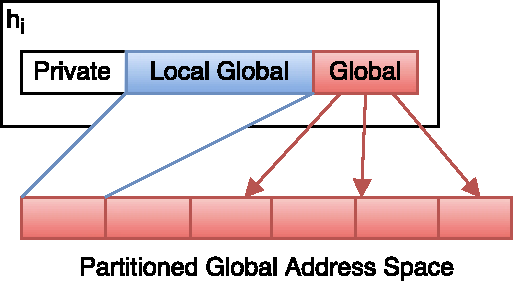
\includegraphics[width=\columnwidth]{Images/BlueBridgeHostMemory.pdf}
    \caption{Illustrations of how global memory is stored in a BlueBridge host.}
    \label{fig:pgas}
\end{figure}
Each machine's memory section contains a private and a global address space (see Figure \ref{fig:pgas}). Private memory is only accessible to critical or privileged processes of the local host, it is not shared with any other node. Global address space is divided into a local and remote section, the former residing physically on the machine.
Local global memory encompasses the address space a server provides for other machines to use, it may also contain memory the host has fetched from remote machines and stored for computation. The global address space is comprised of a collection of pointers the local machine has either reserved from remote hosts or requested for future operations.
% \ugh{All remote memory addresses are mapped locally using the \texttt{mmap()} call and accessed on demand} \hl{needs to be verified}. 
In order to preserve locality, hosts are aware of the global memory available on the machine and all operations are performed locally. In case of a remote fetch, data is written back to the original host. In a scenario involving disaggregated memory and servers acting as memory banks, remote memory will treated as a single uniform address space.
% \subsubsection{The Blueprint}
BlueBridge follows a simple design concept, as shown in Figure \ref{fig:blueprint}.

\begin{figure}[t]
    \centering
    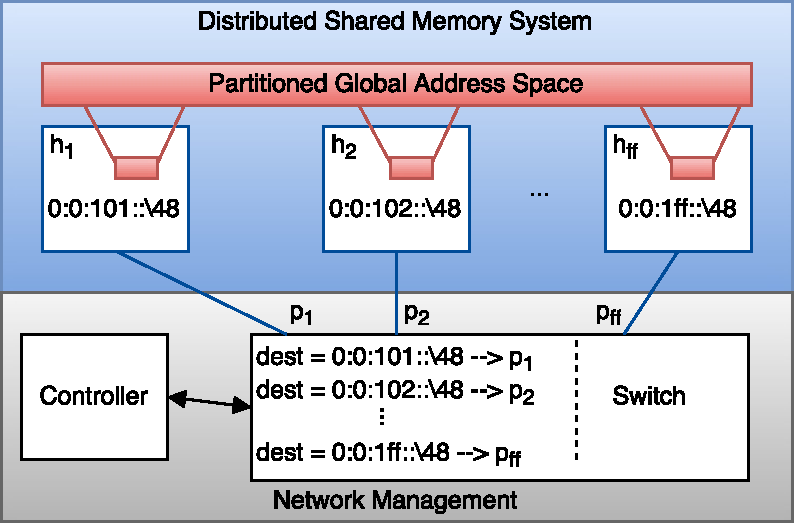
\includegraphics[width=\columnwidth]{Images/BlueBridgeMemory.pdf}
    \caption{High-level blueprint of BlueBridge architecture.}
    \label{fig:blueprint}
\end{figure}

The core of the proposal is a divergence of conventional memory address properties. BlueBridge does not rely on typical PGAS memory design and directly encodes memory addresses as IPv6 pointers. Each client acquires remote memory in the form a 128 bit IPv6-conform address. Instead of storing a request in the payload of a network packet, any subsequent request will be directly inserted into the destination header of the packet.
This design choice allows for powerful operations in the network space which may greatly simplify consistency and coherence management in a DSM system. Any request or operation can be routed, forwarded, copied, or modified directly without hosts being required to track state. Both receiver and sender remain fully unaware of the remote location or current state of the memory as these operations are handled by dynamic network functions.

To support the architectural concept we utilize a software-defined switch as well as controller handling all required operations. To avoid overloading the switch, entries are kept minimal. Servers are assigned a subnet range which represents a global memory partition. In combination with the pointer address, this subnet range creates an unique identifier in the packet header. 

If a client performs an operation requiring the use of a remote pointer, it will insert the stored pointer into the destination IP field of the IPv6 header and send the packet. Since the header contains the unique node ID, the switch is able to instantaneously forward the packet to the correct port. The server will extract the pointer and specific command out of the destination header, perform the specified operation, and reply to the source IP of the packet (which is the unique ID of the client). A client ``keeps track" of an address by extracting the source ID identifier of the replying owner.
Neither server nor client are required to store any information about the location of other machines. For $n$ servers the switch only has to maintain $n$ basic routing entries, mapping each subnet to a specific port.
\newcommand\ipsample{{"0","0","0","0","0","0","0","0","0","1","0","3","0","3","0","0","d","0","8","4","9","5","0","1","0","0","0","0","0","0","0","0"}}

\begin{figure*}
\hspace*{-10px}
  \begin{tikzpicture}[scale=0.55]
    \foreach \x in {0,...,31}
		\node at (\x+0.5,0.25) {\footnotesize \x};
	\foreach \x in {0,...,32}
    \draw[thick, blue] (\x,0) -- (\x,0.5);
    \node[thick] (bit1) at (-0.6,0.24) {\scriptsize nibble};
	\draw [thick] (-1, 0.5) -- (-0,0.5);

    \node[thick] (bit1) at (-0.5,2.25) {\scriptsize IPv6};
	\draw [thick] (-1, 2) -- (-0,2);

	\filldraw[thick,draw=black, fill=white] (0,0.5) rectangle (8,2);
	    \node (mode) at (4,1.25) {\scriptsize IPv6 Scope (Wild Card)};
	\filldraw[thick,draw=black, fill=white] (8,0.5) rectangle (10,2); 
	    \node (mode) at (9,1.5) {\scriptsize BlueBridge};
        \node (mode) at (9,1) {\scriptsize Prefix};
	\filldraw[thick,draw=black, fill=white] (10,0.5) rectangle (12,2);
	\node (mode) at (11,1.5) {\scriptsize Machine};
	\node (mode) at (11,1) {\scriptsize ID};
	\filldraw[thick,draw=black, fill=white] (12,0.5) rectangle (14,2);
	    \node (mode) at (13,1.5) {\scriptsize BlueBridge};
	    \node (mode) at (13,1) {\scriptsize Command};
	\filldraw[thick,draw=black, fill=white] (14,0.5) rectangle (16,2);
	    \node (mode) at (15,1.25) {\scriptsize Arguments};
	\filldraw[thick,draw=black, fill=white] (16,0.5) rectangle (32,2);
	    \node (mode) at (24,1.25) {\scriptsize 64 Bit Pointer};

	%\filldraw[thick,draw=black, fill=white] (0,2) rectangle (32,2.5);
	\foreach \x in {4,8,12,16,20,24,28}
	    \node at (\x,2.25) {\footnotesize \textbf{:}}; 

	\foreach \x in {0,...,31}
        \node at (\x+0.5,2.25) {\footnotesize \textbf{{\pgfmathparse{\ipsample[\x]}\pgfmathresult}}};
\end{tikzpicture}
\caption{The IP destination structure. The top row represents a sample IPv6 
request which is mapped to the structure below.}
\label{fig:ipv6}
\end{figure*}

\subsection{Operations}

The client library currently consists of simple CREATE, READ, UPDATE, DELETE (CRUD) functions for a higher-level application to utilise. The current operational plan for each procedure is as follows:

\paragraph{\textbf{CREATE}}
If a client needs to allocate or reserve a remote memory section, it will call CREATE. The function selects a random ID of the available server range and sends a IP packet containing the create command and destination ID. The switch forwards the packet to the corresponding server. After allocation of a local pointer has been successful on the server side, it stores the address in the payload of the packet and responds with an ACK message. The client will extract the pointer as well as the unique identifier of the server, merge the structure into a unique global pointer, and store it for future use.

The size of a single allocate operation is limited to 4096 byte pages. It may be beneficial to allow clients the specification of arbitrary allocation size. If the size exceeds a certain threshold, both parties can switch to a TCP connection for more efficient data transfer.

For future work, we are considering to render clients fully agnostic of the destination and introduce load-balancing capabilities on the switch. Clients will send generic CREATE destination requests, which will be distributed by the software switch based on optimal locality or load. This approach is possible as the switch is able to forward the generic packet to a controller, which could decide the current optimal placement. It remains to be seen if the trade-off between additional request latency and efficient placement will provide long-term gains.

We are also considering the use of broadcast allocation to inform all other clients of a newly available memory address. Information about the location of shared variables can thus be quickly spread through the network.

\paragraph{\textbf{WRITE}}
Once a client has acquired a pointer, it is able to write to the remote address by inserting the IPv6 structure into the packet header and coupling it with an WRITE command. Data that is to be written is encapsulated in the payload. The server will extract the pointer, store the data of the payload in its global address space, and acknowledge to the client that the operation has been successful. We are currently intending to support three different types of write commands natively.
\begin{itemize}
    \item \textit{Allocate Writes.}
    The client will insert a ALLOCATE-WRITE command in the header as well as the data content in the payload. The server will write the data to its local memory and provide the allocated memory address to the client.
    \item \textit{Blind Writes.}
    Blind writes are simple asynchronous operations unaware of any consistency or coherence semantics. The content of a blind-write packet is directly written to the server disregarding any that has been previously stored in the block. Applications may use this type of write at their own risk.
    \item \textit{Updates.}
    Updates are transactional procedures which guarantee data consistency and correctness. An update operation requires a READ before being able to write data. Update operations transfer ownership temporarily to the accessing node. Further semantics are described in the READ section.
\end{itemize}

\paragraph{\textbf{READ}}
A READ operation is functionally similar to the WRITE call. The server will extract the pointer, store the memory content in the payload, and send the data to the client.

In a concurrent and asynchronous implementation involving direct memory access it may occur that an other client has fetched the same memory and is currently modifying the data block. Our approach to solve this potential race condition is as follows:

As soon as a client has requested an UPDATE operation on a particular memory address, the switch will install a temporary redirect route forwarding all subsequent requests to the current owner of the memory section. The new owner may either reject or process the requesting, depending on the consistency policy of the system or application. To prevent stale reads before the redirect is updated, the server will invalidate its memory section until the client has rewritten the data. After a successful procedure, all temporary flows are removed and data exchange continuous as usual.

\paragraph{\textbf{DELETE}}
A DELETE operation is a simple \texttt{free} or \texttt{memset(0)} operation on the server side depending on desired outcome. If the memory is to be re-used, it can be set to zero, if it is supposed to be deallocated, it can be freed. The client can call DELETE at any time. To prevent the remaining machines from using a stale pointer we are planning to utilise a broadcast message containing the memory address in question. The switch forwards the message to all machines in the network and any affected client will invalidate its pointer.


All of these operations are are stored in the IPv6 header of the packet encoded as single byte, providing a total of 127 unique commands. Storing commands in the header also allows the central coordinating switch to reroute or reject packets based on the nature of the request without involving a server. This feature also opens up the possibility of the control plane to monitor the computational state of the system and interject if necessary.

\subsection{Control Plane}
As the majority of management and coordination operation are shifted into the network, the controller as well as the software switch have to be able to bear a significant amount of computation and load.
The amount of network nodes a packet traverses until its destination has to be minimal. Avoiding a flow table "cache miss" is desired as much as possible is desired as flow-table updates are expensive. These aspects require a proactive flow-installation system and the controller to have global knowledge of the memory layout. Flow table entries in the switch need to cover most common events.
% \paragraph{\textbf{Routing}}
In the default case, the controller will monitor active nodes in the system and proactively install corresponding flow entries. Any packet that matches a particular IPv6 CIDR address will be forwarded to the owner without any further overhead.
\paragraph{\textbf{Update operations}}
\label{par:updates}
Update operations require consistency which can be enforced by the control plane. For any header containing an UPDATE command, the switch will forward the packet to the node as well as the controller to process.
The packet will trigger the controller to call a flow-table update procedure which will install a redirect entry of the specific pointer address to the new owner.
In order to mitigate the exhaustion of flow tables, these entries must be temporary.
After installing the flow rule, two possible events may occur. Either the client writes the content back to the original
node and triggers a new controller action to delete the entry, or the flow expires. If a flow expires, the controller as well as server assume that the client operation has failed and the memory section is marked available again. The delayed write operation of the client will be rejected. 


\paragraph{\textbf{Monitoring}}
Port mirroring of switch traffic as well as out-of-band monitoring and management of client machines allow for a comprehensive central view of the controller of all network events. Opportunities may include fast-failover in case of single machine failure, or identification and dynamic rebalancing of hot memory partitions.

In addition to conventional strategies, a realizable migration concept may include live-updating of flow entries to move traffic to less active nodes. As the switch is able to route by inspecting commands in the destination header, it is possible to redirect WRITE operations to a different host. After successful completion, the controller will install a permanent flow entry redirecting requests to the new owner.
A client thus incidentally and seamlessly migrates data while keeping the data flow of the system intact.
One significant drawback of this method is the eventual fragmentation and subsequent switch table exhaustion. 
Consequently, we intend to assess and thoroughly evaluate the feasibility and computational complexity of specific procedures leveraging these two properties.

\paragraph{\textbf{Controller performance and flexibility}}
The control plane is a crucial component of the BlueBridge system. As it primarily rests upon the underlying controller architecture, we require a mature, efficient, and reliable framework.
Potential candidates under investigation include Beacon, Nettle, OpenDaylight, and ONOS. While ONOS~\cite{onos} and OpenDaylight~\cite{odl} are comprehensive frameworks with a multitude of features and industry support, they are comparably slow.~\cite{controller_perf1} Beacon~\cite{beacon} and the Nettle language~\cite{controller_perf2} feature extremely fast processing and response times, but are largely academic. Beacon is not under active development and Nettle is written in Haskell with unclear maturity and flexibility. 
BlueBridge is tightly coupled to the capabilities of the control platform and we have to weigh benefits of each control plane paradigm. Opting for the right framework is essential for the system to succeed.

% \subsection{Discussion}
% Although BlueBridge is still in the prototyping stage, particular limitations and properties of the design may be fundamental.

% \subsubsection{Switch and Controller Performance}
% It is unclear, if hardware switches and control software are capable of handling the update frequency demanded by the current design.
% Complex operations such as migration or updates may quickly exceed maximum switch performance and flow table efficiency. Evidence suggests that software switch tables are easily exhausted under heavy load.~\cite{controller_perf1,controller_perf3}
% If and only if the flow table size, updates,  and expiration times are kept sufficiently small, we can expect the system to remain stable.
% \subsubsection{Managing a Dynamic Address Space}
% Migrating and splitting memory partitions of the global address space introduces substantial complexity. In our design, a memory address is a unique heap pointer exclusive and only correct on the machine it has been allocated in. A redirected client access as described in section \ref{par:updates} will lead to incorrect access or corruption on a different machine. Maintaining a specific mapping on either the client or server side is costly and violates the agnostic end-host principle of BlueBridge. A potential solution is to notify the client to update its allocated memory address using either over broadcasts or specific controller messages. The client will update its mapping with the pointer and source address of the new owner, preserving correctness in the system.

% \subsubsection{Designing for failure tolerance and scalability}
% BlueBridge is built around one single switch maintaining all flow tables on rack-scale, interacting with a single controller. It is an open question to what level the system should be fault-tolerant, if at all. While it is feasible to mirror the controller as well as the switch without incurring too much overhead, it may be costly. Failure-tolerance may be pushed to applications to reduce configuration and operational complexity.
\section{Proof of Concept System}
\label{sec:implementation}
To evaluate the practicality of the aforementioned design we built a simple proof-of-concept tool operating entirely on IPv6 memory addressing. The implementation is minimal and focuses on appropriate conversion and network transport techniques to demonstrate the basic IPv6 shared memory use case and its benefits. The virtual memory system as well as the control plane and consistency management properties of the BlueBridge design are left as future work.
The client-server program is written in C and Python and utilizes basic C memory operations.
\subsection{System Aspects}
% The general operational structure of the tool is already reminiscent of the full design proposal.
The client consists of a library of simple remote allocate, read, write, and free functions which are mirrored on the server side. Allocation is chosen at random out of a list of possible host numbers. Instead of \texttt{mmap()}, the client stores acquired pointers in a simple list structure to read and write its data. When accessing remote memory the client inserts the IPv6 pointer into the header and sends it using a Linux datagram socket. The server retrieves the destination IP section, converts the 128 IPv6 address into a 64 bit pointer, and faithfully performs the requested action. We currently do not check for invalid or corrupted pointer addresses, which may lead to errors on the server side. A fully asynchronous, non-blocking client and server programs as well as checking pointer addresses are functions left for future work

\subsection{Networking Aspects}
We run our proof of concept system in Mininet~\cite{mininet}, a networking virtualization engine primarily used for SDN research.
% It enables the testing of networking configurations on a single machine by encapsulating nodes in a custom, dedicated network container.
% Mininet supports virtual switches as well as custom controllers, making it a prime candidate to conduct our tests.
Our current network setup consists of a single switch and controller managing up to 42 nodes. We are running a simple Open vSwitch which is pre-configured over several static \texttt{add-flow} commands which specify the appropriate server subnets. 
% Although the system is capable of running in conjunction with a controller (here: Ryu), we are not yet relying on it. The controller would only operate in reactive mode and not install any routing entries. 
All forwarding is performed on layer two only and all flow entries are MAC-based. As these type of operations can be just as effectively covered by the static configuration, we have decided to not include the controller in this prototype.We leave controller integration to future work.

We still rely on the Linux network stack for communication, which automatically configures all necessary operations below transport layer. This includes neighbor discovery, packet construction, route entry management, and packet forwarding.
Every pointer is a unique IPv6 address and hosts do not reply to unknown addresses. As a consequence, our system needs dedicated routing table entries for each node and utilize the network discovery protocol to function properly.
As it is impossible to specify IPv6 subnet proxies natively, every node runs a NDP-proxy server which responds to NDP solicitation requests. For every pointer that is sent out into the network, a NDP solicitation request is broadcast. The proxy of the owning server will respond and the appropriate routing entry is created on all relevant nodes.
This behaviour is highly undesirable as it generates round-trip overhead, nearly doubles network traffic, and may lead to peculiar problems (see Section~\ref{sec:silly_ndp}). It is thus mandatory to abolish the dependence on NDP for our system to succeed. As it is a default feature of Linux transport layer operations, we are planning to move to raw socket programming entirely. This also provides us with the benefit of high customizability and the potential to define a leaner, specialized protocol.

\subsection{IPv6 Remote Paging}
% \ac{Amanda please work on.}
% \ac{Done to be similar to DSM systems work, see \cite{Protic1996}}
We also created a \texttt{userfaultfd} program to perform remote paging, reminiscent of how DSM systems would transparently retrieve remote memory for an application. When a page fault occurs, the system determines if the page is remote or local. If the page is remote, it performs whatever communication is necessary to retrieve it, if it is local, it fetches the page. \cite{Protic1996} In our implementation, we moved most of the \texttt{client} logic into \texttt{userfaultfd}. The program \texttt{mmap}s $n$ number of addresses into memory marked to be handled by the \texttt{userfaultfd} handler. When it \texttt{mmap}s the memory, it allocates remote memory on the \texttt{server} and maintains a mapping of local addresses to remote addresses. Every access causes a page fault which is handled by our handler. We then forced page fault accesses to these pointers. For each page fault, the program checks to see if the pointer is remote or not by checking a hardcoded map. If the pointer is remote, it performs a READ operation on the remote memory and loads that into the local pointer.

% After building the program we conducted several tests to evaluate its current efficiency and to identify potential shortcomings and bottlenecks.

%%%%%%%%%%%%%%%%%%%%%%%%%%%%%%%%%%%%%%%%%%%%%%%%%%%%%%
\section{Evaluation}
\label{sec:eval}
% \ugh{ASSIGNED TO: Amanda}\\
%%%%%%%%%%%%%%%%%%%%%%%%%%%%%%%%%%%%%%%%%%%%%%%%%%%%%%
% \ac{Outline:
% \begin{itemize}
%     \item Quick explanation as to what this eval shows
%     \item Explain the experiment setup. This should discuss mininet and how the programs measure things and where
%     \item Explain the remote paging latency
%     \item Explain the RDMA speed up compared to disk
% \end{itemize}}
% Our proof of concept shows that IPv6 addressed memory is possible, but one critical aspect that must be evaluated is the overhead incurred by remote paging. 
We evaluate our implementation in two ways. First, we look at the simulated speed up with a directory service switch to determine the overhead improvement our design brings. Next, we consider how the overhead compares to disk access if the communication used is RDMA. 


\subsection{Experimental Setup}
As mentioned in Section \ref{sec:implementation}, we used Mininet to simulate the network and switch for our tests. In our evaluation, we have three hosts, three servers, three NDP proxies, one switch, and one controller. Mininet was run on a machine with an Intel(R) Core(TM)2 Quad CPU Q9400 @ 2.66GHz, 4 GB of memory, and the mininet configuration reached a peak bandwidth of about 800 Mbits/sec. Each experiment was measured in nanoseconds, when the median latency and 95th percentile were calculated, the latencies were then converted into $\mu$s.

As mentioned before, this implementation uses a static switch configuration (learning switch). Although this makes our performance numbers not entirely representative of our proposed design, it does provide a good indication as to how the system will perform once it is fully built. 

% \ac{Would this be better in the implementation section? Is it even necessary?} We measure latency using the \texttt{timespec} struct in C and \texttt{clock\_gettime$\left(\text{CLOCK\_MONOTONIC,...}\right)$}. Our latency measurements are taken in nanoseconds and, when analyzed, they are converted into $\mu$s. 

\subsection{Remote Paging Latency}
% \ac{Outline:
% \begin{itemize}
%     \item Reiterate main goal of proof of concept: to show feasibility of IPv6 addressing
%     \item Claimed improvement --> reduced overhead due to one less RTT
%     \item But how much will that actually improve things?
%     \item Explain experiment setup (i.e., 1500 pages, userfaultfd program, not actually doing a remote write, etc.)
%     \item Discuss total latency comparison first
%     \item Discuss read and write breakdown, highlight how the RTTs are the worst part of the latency, therefore removing one makes a huge impact. 
%     \item Segway into RDMA discussion
% \end{itemize}
% }
One of the main benefits of moving the management into the switch is the improved performance. This improved performance comes from reducing a roundtrip time (RTT) to the directory service. But this assumes that the RTT to a directory service incurs enough cost to affect the overall latency. To explore this, we simulated three scenarios: 1) shared memory system with a centralized directory service, 2) shared memory system with a directory service in the switch, and 3) a normal system disk access. We include the disk access in our measurements to provide a baseline for comparisons. We do not claim that we currently outperform a disk access, although our performance numbers point to the ability to do so with proper optimizations.

The shared memory system with a centralized directory service (Remote w/ DS) is simulated by querying the server for the IPv6 address of a piece of memory it requires to access. The server will then respond with an IPv6-compliant pointer for the client to use in a READ request. The shared memory with a directory service in the switch (Remote w/o DS) stores the IPv6-compliant pointer when allocating the memory, thus allowing it to skip the step of asking a directory service which machine to send its pointer to. This is not our exact design, as we would have a rule in the switch which recognizes which machine to send this pointer. It will be similar in overhead cost because it does not query the directory service. 
% A decentralized shared memory platform would behave similarly, but only because it requires communication when memory moves, not on every access. Since we do not have a controller implemented for our solution, we do not compare to the decentralized shared memory, we save this for future work. 
The normal system disk access (Local) reads a dummy file from disk and loads it into memory. 

We ran each program with 1,500 pages, where it accesses each page once. We record the latency at multiple points of the execution path to determine where each program spends most of its time as well as the total latency. We then graph the median of these latencies with the 95th percentile error bars. The total latency is shown in Figure \ref{fig:total_latency} and appears as expected. The Remote w/ DS performs the worst and the disk access performs the best. We expected the disk access to perform the best because we did not optimize our proof of concept to use RDMA, therefore avoiding the server CPU. We discuss the implications of using RDMA in the next section.

\begin{figure}[t]
    \centering
    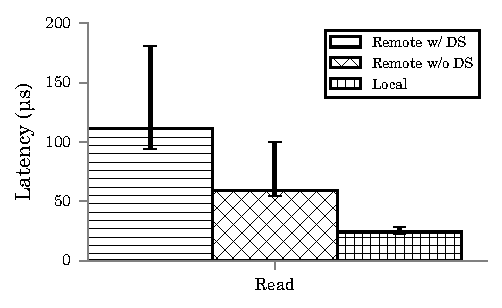
\includegraphics{Graphs/Latency_Total_Comparison.pdf}
    \caption{A comparison of the total latency per page fault of reads under three conditions: remote read with a directory service call, remote read without a directory service call, and accessing local disk. This is the median latency over 1,500 accesses of different pages with 95th percentile error bars.}
    \label{fig:total_latency}
\end{figure}

We breakdown the total latency into five categories: enter handler, exit handler, access DS (directory service), get data, and other. Enter handler is the amount of time it takes from the application level access of a page which faults till the handler receives the event notification. Exit handler is the time it takes after the handler finishes its work till the application is no longer blocked. Access DS is the amount of time the handler spent querying the directory service for the machine to send the request to. Get data is the amount of time the handler spends getting the data from the remote host or disk. 

The interesting part of the latency breakdown, Figure \ref{fig:read_breakdown}, is how much time the Access DS and Get data take compared to the other operations, they take approximately 9x longer. Based on that, it's obvious that reducing the execution path to one RTT instead of two is desirable. The reason the RTTs are drastically slower is the fact that we perform all communications over UDP on Ethernet. If these operations were done with RDMA, there should be a more significant speed up.

\begin{figure}[t]
    \centering
    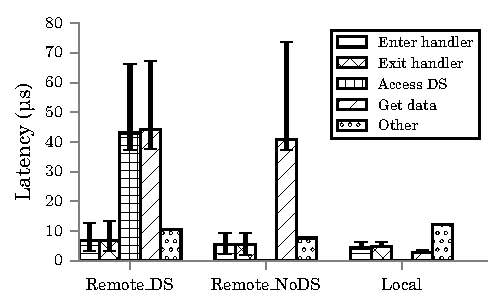
\includegraphics{Graphs/Latency_Breakdown_Read.pdf}
    \caption{A breakdown of the latency cost for a read under three conditions: remote read with a directory service call, remote read without a directory service call, and accessing local disk. This is the median latency over 1,500 accesses of different pages with 95th percentile error bars.}
    \label{fig:read_breakdown}
\end{figure}

% \begin{figure}[t]
%     \centering
%     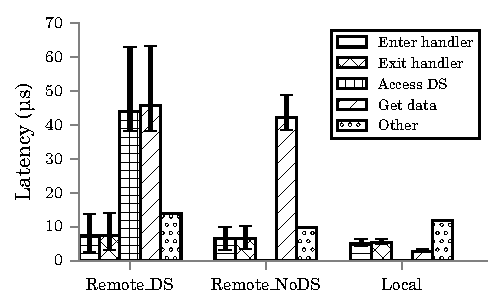
\includegraphics{Graphs/Latency_Breakdown_Write.pdf}
%     \caption{A breakdown of the latency cost for a write under three conditions: remote write with a directory service call, remote read without a directory service call, and accessing local disk. This is the median latency over 1,500 accesses of different pages with 95th percentile error bars.}
%     \label{fig:write_breakdown}
% \end{figure}

\subsection{Potential Gains of RDMA}
% \ac{Need better subsection title.}
% Outline:
% \begin{itemize}
%     \item As seen above, there is something to gain from removing the directory service, but still much higher latency than disk.
%     \item Well, original design uses RDMA, so how much will it improve things?
% \end{itemize}
% }
Most modern shared or remote memory systems leverage RDMA. Due to time constraints we could not leverage it for our proof of concept, but we still consider it in our performance evaluation. In our latency breakdown, we found that the RTT costs approximately 9x more than any of the other operations, which indicates that moving the directory service into the switch is very beneficial. But, we performed all communication in a non-optimal way, therefore we compare the amount of time it takes each remote operation with our communication method (UDP) and the equivalent RDMA method.

We have four operations, as stated in Section \ref{sec:overview}, CREATE, READ, UPDATE, DELETE. The RDMA equivalent for READ and UPDATE is RDMA read and RDMA write, respectively. CREATE and DELETE can be achieved using RDMA send/recv to issue commands to the remote server. According to experiments done by Ma et al. and Zhu et al., the approximate cost for an RDMA read or write operation is 3.4 $\mu$s and the approximate cost for an RDMA send/recv is 5.6 $\mu$s~\cite{Ma2016, Zhu2015}.\footnote{Reported latencies were one-way latencies for 2k and 4k pages. We doubled the reported latencies to make them roundtrip} We measured the latency of a small RDMA cluster using \texttt{qperf} to get one-way latencies for 4096 bytes. They mainly aligned with the numbers reported in \cite{Ma2016, Zhu2015}, so we use them in Table \ref{table:rdma_compare}.

As seen in Table \ref{table:rdma_compare}, using RDMA primitives instead of UDP improves the roundtrip time by 6x. Even with the improved communication latency, accessing a remote directory service incurs a high cost. In the worst case, it uses UDP and adds 45 $\mu$s, in the best case it uses RDMA primitives and adds 5.84 $\mu$s. It is still unnecessary overhead which can be mitigated by moving the directory service into the switch.

Another interesting observation of using RDMA, is that the theoretical latency would bring the total latency of our proposed solution into the same range as local disk. Our solution with the theoretical RDMA latency would cost approximately 22.116 $\mu$s, whereas the local disk latency is 24.304 $\mu$s.

\begin{table}[t]
    \begin{tabular}{ | l | l | l | l | }
        \hline
        & UDP ($\mu$s) & RDMA ($\mu$s) & Speed-up (x) \\ 
        \hline\hline
        Create & 34.919 & 5.84 & 5.979\\
        \hline
        Read & 33.732 & 5.92 & 5.698\\  
        \hline
        Update & 34.151 & 5.96 & 5.730\\
        \hline
        Delete & 32.963 & 5.84 & 5.644\\
        \hline
    \end{tabular}
    \caption{Comparison of our communication operations vs. their RDMA equivalent. For READ and UPDATE, the equivalents are RDMA read and write. For CREATE and DELETE, the equivalent is RDMA send/recv. Our latency medians were gathered over 1,500 runs of each operation. The RDMA measurements were gathered using \texttt{qperf}.}
    \label{table:rdma_compare}
\end{table}


% \begin{figure}
%     \centering
%     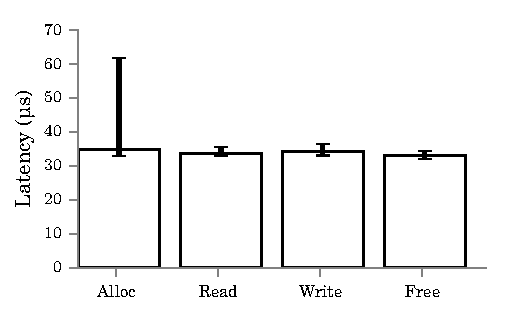
\includegraphics{Graphs/Microbenchmarks_Latency.pdf}
%     \caption{The median latency cost of each remote operation over 1,500 calls with 95th percentile error bars.}
%     \label{fig:micro_latency}
% \end{figure}

\subsection{Data Migration}
We attempted to perform data migration in our proof of concept system. Unfortunately, due to the NDP proxies required and the current network setup, data migration did not work. The switch was able to re-route the packets and the memory could easily be allocated at the same address on the new host server using \texttt{mmap()}, but the packets were getting dropped by the Linux network stack on the receiving server. This is because they were coming from an unknown address. Our system circumvents this issue by using the NDP proxies, but these do not work in the data migration case. Once we build a system which uses raw sockets and does not rely on NDP proxies, we will evaluate the data migration. We believe that data migration will work once the networking issues are fixed. 

\subsection{Observations}
While running our tests we made several interesting observations.

\subsubsection{NDP Table Exhaustion Attack}
\label{sec:silly_ndp}
As we increased the number of pointers to access we noticed our program continuously deadlocking around the 1000th to 1500th iteration. The packet of the client never reached its destination. However, neither server nor client showed signs of exhaustion and race conditions were unlikely due to the strictly sequential nature of the program. We initially suspected the switch to overload and drop packets, but the device forwarded correctly. The actual fault occurred on the client side. Although the \texttt{send()} system call of the program returned correctly without error, the packet was never forwarded to the interface. The cause of this issue was the NDP neighbor table on the client host. The client accidentally performed a NDP Table Exhaustion Attack~\cite{RFC3756} (see Figure \ref{lst:ndp_err}) on its own NDP neighbor table. The protocol generates a mapping for every unique IPv6 address to the destination interface. While the client allocates several thousand pointers, several thousand entries are created in the table. By default Ubuntu's NDP tables only have a size of around 4096 byte and the values expire slowly. The table is quickly exhausted and no entries can be created, which leads to a packet being quietly dropped and the program stalling. It seems that the only effective mitigation technique is to increase table size. NDP Neighbor tables do not seem offer netmask level matching nor is it possible explicitly specify a expiration time lower than 1 second. This is a crucial design flaw and further motivation to abolish NDP in our system. As we are moving towards raw socket messaging regardless, we are, as of this moment, not concerned about this problematic behavior.

\begin{figure}
\parbox[b][12px][t]{0.45\textwidth}{
 \footnotesize
 \texttt{[46768.440041] neighbour: ndisc\_cache: neighbor table overflow!}\\
 \texttt{[46770.564832]~neighbour: ndisc\_cache: neighbor table overflow!}\\
 \texttt{[46770.580728] neighbour: ndisc\_cache: neighbor table overflow!}
 } 
\caption{NDP table exhaustion error messages.}
\label{lst:ndp_err}
\end{figure}
\subsubsection{Mininet Performance Limits}
Initially we planned to test the rack-scale scalability of our system on Mininet. However, we faced limitations regarding the physical resources of our test machines. We conducted the tests on a Ubuntu 16.04 LTS machine with 12GB of RAM and a four-core i5 760 @ 2.80GHz processor. The first test involved launching 42 hosts, each running a client/server process as well as ndp-proxy daemon. Each client performed a 100 full iterations, but the test did not complete as several clients froze

In the second test, a single client performed a 1000 full iterations. The client also froze. 
A 42 unit Mininet cluster significantly stresses the CPU of the host system, thus it is unclear whether these results are due to Mininet's scalability constraints or design flaws in our system.
In addition, NDP seems to be a significant contributor to the load on the system. As every system maintains neighbor discovery, new pointers create solicitation storms across all nodes.
We plan to retry these tests after implementing raw socket messaging.

\subsubsection{Disk Access Latency} The reported disk access latency numbers (Local in Figure \ref{fig:total_latency}) are much lower than previously reported disk access latencies in literature. This is due to the file being accessed from the buffer cache instead of the disk every read. Since the page fault handler reads the same file, at the offset of 0, the file's content is most likely stored in the buffer cache instead of causing a disk seek every access. We plan to re-run the tests in future work with a larger file, random offsets, and buffer cache flushing to ensure that the file is read from disk every page fault.
% \fr{\\Does flushing the buffer cache not work?\\ https://unix.stackexchange.com/questions/87908/how-do-you-empty-the-buffers-and-cache-on-a-linux-system\\
% https://www.chrisnewland.com/clear-linux-buffers-cache-when-benchmarking-filesystem-337}
% \ac{It does, but I don't have the time to implement it. }
% %%%%%%%%%%%%%%%%%%%%%%%%%%%%%%%%%%%%%%%%%%%%%
\section{Discussion}
\label{sec:discussion}
%%%%%%%%%%%%%%%%%%%%%%%%%%%%%%%%%%%%%%%%%%%%%

\textbf{Using Dinv.} Dinv infers invariants that are \emph{likely}
because it is a dynamic analysis approach that only considers some
finite set of system behaviors. The inferred invariants are not a
verification of the system.
%
But, Dinv is pragmatic when considering today's software development
practices that include widely used dynamic analyses like testing.
%
Unlike testing Dinv helps developers understand what happened. Dinv
can be extended towards testing by having developers assert expected
Dinv-inferred invariants for a set of curated executions.

%% standard practice. Moreover, Dinv can actually augment the results of
%% test runs.

%% we were able to observe it under real
%% world conditions (long runs, failure scenarios) without needing a
%% complete specification of it's behavior.
%% %
%% Dinv allowed us to refine and narrow the instrumentation iteratively
%% based on actual execution results.

To use Dinv a developer must have access to the system's source code,
and they must be familiar with the system. In our evaluation we considered
four large distributed systems, none of which we were familiar with
prior to this study. In each case we used all of the resources
available to us (papers, source code, documentation) to understand the
desired system properties and to interpret Dinv's output. We have not
carried out a formal usability study on Dinv, but we do have some
anecdotal evidence that it is not difficult to use: students with no
prior distributed systems background successfully used it in a
graduate distributed systems course. 

%% Its' behavior, which is often not
%% thoroughly documented, must be translated into \emph{likely
%%   specifications} that we can infer.
%

Depending on design of the system distributed state may be difficult
to identify and encode, particularly when this requires reasoning
about program paths that lead to network actions.
%
As we had no prior knowledge about the four systems in our evaluation
and were successful in inferring interesting properties we are
confident that with proper training developers would be able to
similarly instrument their systems.
%
% However, the catch is that the developer must be willing to and is
% sufficiently familiar with their system to interpret \emph{likely
%  specifications} that we infer for their system.

\textbf{Merging strategies.} Dinv's three merging strategies
(Section~\ref{sec:merging}) were motivated by our evaluation
experience. These cover different views on the systems and allow Dinv
to detect a wide range of invariants, from properties true across all
hosts during the entire execution, to eventual consistency properties
observed on the level of send-receive pairs. Even so, these strategies
are not exhaustive. All three merging strategies were implemented in
less than 15 LOC; we therefore think that custom merging strategies
offer a reasonable way to extend Dinv.

%% The lattice structure provides all data necessary for different
%% analysis approaches.

\textbf{Daikon templates for distributed system invariants.}  Daikon
is designed to infer invariants for program points in a sequential
system. Dinv uses Daikon by presenting it with a synthetic program
point that actually corresponds to a distributed state. This approach
has its limits. In particular, Daikon supports a fixed set of
invariant templates that at most describe 3-ary relations. %This is
%insufficient for mining invariants like the one given earlier:
For an invariant mentioned earlier, $coordinator.commit =
replica_i.commit$ for each replica $i$, Dinv mines as many individual
invariants as there are replicas in the system.
%
%Another approach 
%is to extend Daikon invariant templates to be 
%
We experimented with adding support for n-ary properties to Daikon and
see promising results. These properties would help to compactly
describe properties of larger systems, like those with many nodes.
%% We also added an invariant while
%% trying another approach to checking eventual consistency, by showing
%% that at each point the difference in state between hosts is bounded.

\textbf{Analyzing executions containing failures}. A major challenge
for distributed systems is dealing with failures. In our experiments
with the SWIM protocol in Serf we have shown that Dinv can establish
properties of a system during network partitions. However, in general,
Dinv is limited in the kinds of system failures it can be used to
study.
%
\dinv's decision to split the execution into strongly consistent cuts
and translating the happens-before graph into a lattice structure
assumes a relatively stable execution environment. For example, a run
with a network partition that is not resolved before the end of
execution, may not result in any cuts from the point where the
partitioned occurred. Supporting other failure cases may require
changing \dinv's analyses; a nuanced, but feasible project.

%% , we were able to extract useful knowledge from
%% executions with network failures.
%

%% On the other hand, infrequently communicating nodes will force the
%% lattice to fan out during log analysis which often set's an upper
%% bound on the number of analysed hosts for performance reasons. Further
%% code optimization of \dinv or the application of more advanced
%% algorithms might alleviate this problem. We didn't feel our analysis
%% to be limited by the number of nodes behind a reasonable threshold.

\section{Conclusion}
\label{sec:conclusion}

We have shown and discussed a new version of DSM which leverages in network
management to expose a NUMA machine to the user. This provides a simple
generic interface for the developer to program on, yet still provides the
benefits of distribution of data and compute. We describe the Camelot system,
which builds upon the BlueBridge system by adding multi-threading support,
different paging policies, and RAID for memory fault tolerance. We evaluated
each additions' performance impact and functionality. In our current setup, Camelot was able to scale 
up to eight cores, achieving a throughput of 3.5 Gbps with an average request latency of around 60 
microseconds. In memory RAID cost a 6\%overhead in computation, but required half of the memory of RAMCloud with comprable fault tolerance.


% \section{Acknowledgements}
% Thanks to Mihir for advice and guidance throughout this project and paper writing process.

\bibliographystyle{ACM-Reference-Format}
\bibliography{paper} 

\end{document}
